% Created 2023-03-12 Sun 18:26
% Intended LaTeX compiler: pdflatex
\documentclass[11pt,a4paper,final]{article}
\usepackage[a4paper, total={7in, 10in}]{geometry}
\usepackage{algorithm2e}
\usepackage{booktabs}
\usepackage{hyperref}
\usepackage{subcaption}
\usepackage{graphicx}
\usepackage{tikz}
\usepackage[utf8]{inputenc}
\usepackage[T1]{fontenc}
\usepackage{graphicx}
\usepackage{longtable}
\usepackage{wrapfig}
\usepackage{rotating}
\usepackage[normalem]{ulem}
\usepackage{amsmath}
\usepackage{amssymb}
\usepackage{capt-of}
\usepackage{hyperref}
\usepackage{amsfonts}                       % Cool math fonts
\usepackage{amsmath}                        % Maths
\setlength\parindent{0pt}                   % No indent for paragraphs
\author{Alexander Brown}
\date{\today}
\title{LLL}
\hypersetup{
 pdfauthor={Alexander Brown},
 pdftitle={LLL},
 pdfkeywords={},
 pdfsubject={},
 pdfcreator={Emacs 28.2 (Org mode 9.5.5)},
 pdflang={English}}
\begin{document}

\maketitle
\parskip 3mm                                % Set the vetical space between paragraphs
\let\ref\autoref                            % Redifine `\ref` as `\autoref` because lazy

\section{1}
\label{sec:orgdcc62e3}
\subsection{Question}
\label{sec:orga4da0f4}
Write a MATLAB program that will plot a lattice in the interval [0,40] on the \(x\) axis and [0,20] on the \(y\) axis.a

\subsection{Solution}
\label{sec:org520038d}
\begin{verbatim}
b1 = [10;2];
b2 = [12;5];
b  = [b1 b2];
plattice(b, "one")
\end{verbatim}

Output is shown in \ref{fig:lattice}.

\begin{figure}[htbp]
\centering
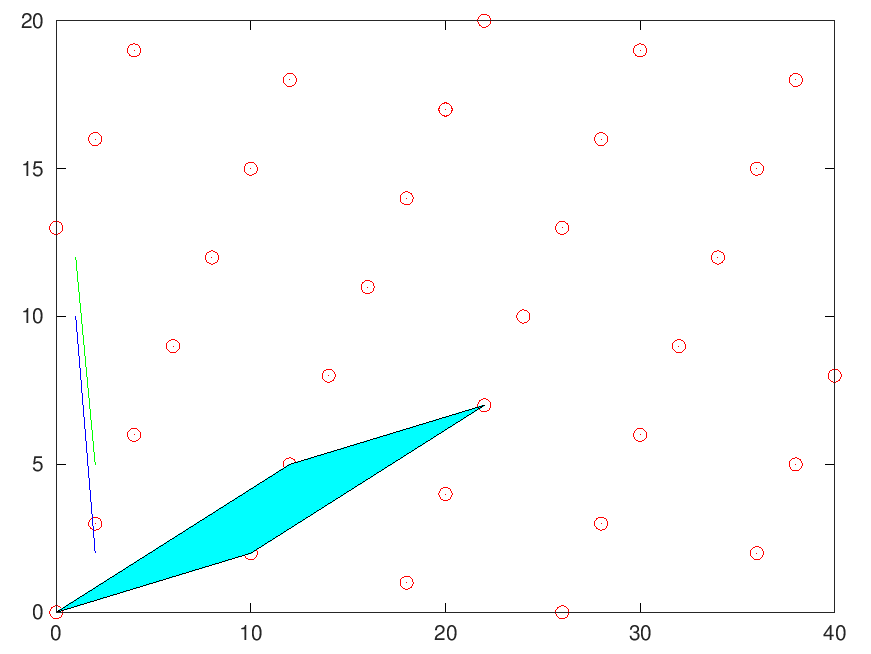
\includegraphics[width=.9\linewidth]{./one.png}
\caption{\label{fig:lattice}Plot of lattice}
\end{figure}

\pagebreak
\section{11}
\label{sec:org66633c0}
\subsection{Question}
\label{sec:org0f5a3b6}
For the basis vectors

\begin{equation}
\begin{array}{cc}
b1 =
\begin{bmatrix}
12 \\ 2
\end{bmatrix}
b2 =
\begin{bmatrix}
13 \\ 4
\end{bmatrix} \\
\end{array}
\end{equation}

verify that the reduced basis vectors are

\begin{equation}
\begin{array}{cc}
b1 =
\begin{bmatrix}
1 \\ 2
\end{bmatrix}
b2 =
\begin{bmatrix}
9 \\ -4
\end{bmatrix} \\
\end{array}
\end{equation}

\subsection{Solution}
\label{sec:orge296260}

\begin{verbatim}
b1 = [12;2];
b2 = [13;4];
b  = [b1 b2];
LLL(b,true);
\end{verbatim}

\begin{center}
\begin{tabular}{rr}
1 & 9\\
2 & -4\\
\end{tabular}
\end{center}

\begin{figure}[htbp]
\centering
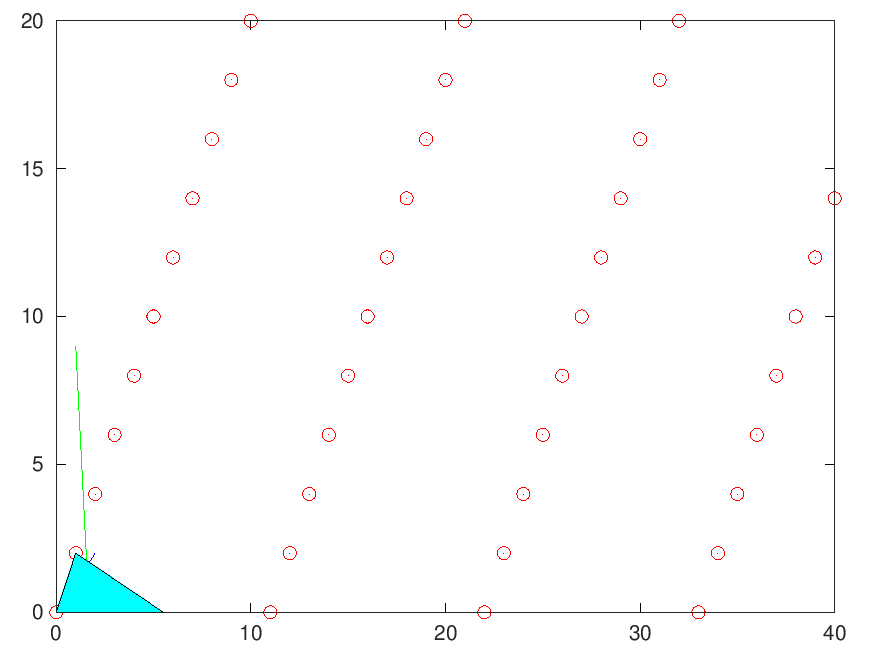
\includegraphics[width=.9\linewidth]{./lattice.png}
\caption{\label{fig:reduced}Plot of reduced lattice}
\end{figure}

Output is shown in \ref{fig:reduced}

\pagebreak
\section{12}
\label{sec:orgd2989d7}
\subsection{Question}
\label{sec:org1d079c2}
\begin{equation}
B =
\begin{bmatrix}
1 & -1 & 2 \\
1 & 0 & 5 \\
1 & 2 & 6
\end{bmatrix}
\end{equation}

verify that the reduced basis vectors are

\begin{equation}
B =
\begin{bmatrix}
0 & 1 & -2 \\
1 & 0 & 0 \\
0 & 1 & 1
\end{bmatrix}
\end{equation}

\subsection{Solution}
\label{sec:org6321ee5}
\begin{verbatim}
B  = [1, -1, 3;
      1, 0,  5;
      1, 2,  6];

LLL(B,false);
\end{verbatim}

\begin{center}
\begin{tabular}{rrr}
0 & 1 & -2\\
1 & 0 & 0\\
0 & 1 & 1\\
\end{tabular}
\end{center}

\section{13}
\label{sec:orgdb9724d}
\subsection{Question}
\label{sec:org94dca37}
\begin{equation}
B =
\begin{bmatrix}
1 & 0 & 0 & 0 & 0 & 0 & 0 \\
0 & 1 & 0 & 0 & 0 & 0 & 0 \\
0 & 0 & 1 & 0 & 0 & 0 & 0 \\
0 & 0 & 0 & 1 & 0 & 0 & 0 \\
0 & 0 & 0 & 0 & 1 & 0 & 0 \\
0 & 0 & 0 & 0 & 0 & 1 & 0 \\
-366 & -385 & -392 & -401 & -422 & -437 & 1215 \\
\end{bmatrix}
\end{equation}

verify that the short vector

\begin{equation}
b1 =
\begin{bmatrix}
0 & 0 & 1 & 1 & 1 & 0 & 0
\end{bmatrix}
\end{equation}

is obtained.

\subsection{Solution}
\label{sec:org1459751}
\begin{verbatim}
B = [1 , 0 , 0 , 0 , 0 , 0 , 0 ;
     0 , 1 , 0 , 0 , 0 , 0 , 0 ;
     0 , 0 , 1 , 0 , 0 , 0 , 0 ;
     0 , 0 , 0 , 1 , 0 , 0 , 0 ;
     0 , 0 , 0 , 0 , 1 , 0 , 0 ;
     0 , 0 , 0 , 0 , 0 , 1 , 0 ;
     -366 , -385 , -392 , -401 , -422 , -437 , 1215]

LLL(B,false);
\end{verbatim}

\begin{center}
\begin{tabular}{rrrrrrr}
0 & 0 & 1 & 0 & -2 & 0 & 5\\
0 & 1 & 0 & 2 & 1 & 1 & 2\\
1 & 1 & 1 & -1 & 1 & -1 & 2\\
1 & 0 & -1 & 1 & -1 & -1 & 0\\
1 & 0 & 1 & 0 & -1 & 2 & -1\\
0 & 1 & 1 & 1 & -1 & -1 & -4\\
0 & 1 & -1 & -1 & 0 & 1 & 1\\
\end{tabular}
\end{center}

\section{14}
\label{sec:org704e8a5}
\subsection{Question}
\label{sec:orgd52a9ea}
\subsection{Solution}
\label{sec:orge4a3859}
The result from \texttt{hackerman.m} is "]".

\begin{verbatim}
hackerman
\end{verbatim}

\begin{verbatim}
]
\end{verbatim}
\end{document}
